\section{The research problem and its outcome}
\label{sec:problem}

\begin{figure*}[t]
  \centering
  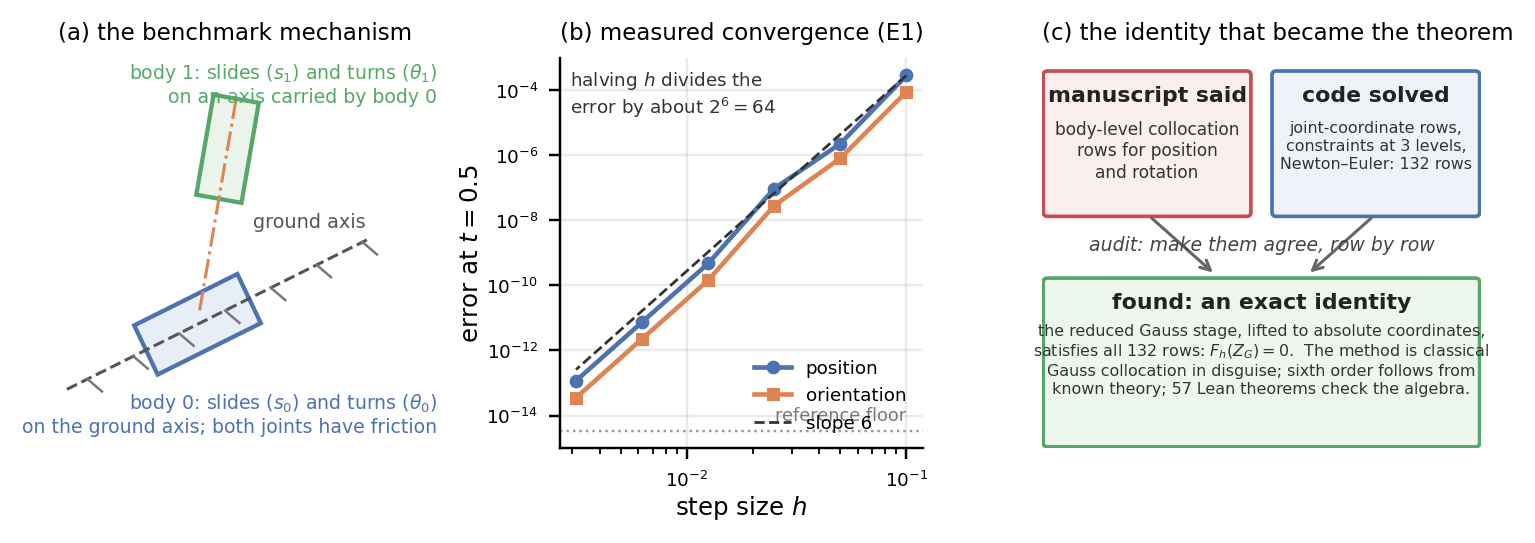
\includegraphics[width=\textwidth]{figures/fig_problem.png}
  \caption{The research problem and what came out of it. (a)~The benchmark: two rigid bodies, each
  sliding and turning on an axis, with friction in both joints. A time integrator advances all
  positions, rotations and velocities by a step $h$ while keeping the joints exactly closed.
  (b)~The measured error of the final method on this benchmark at $t=0.5$, from the E1 result file:
  the slope of $6$ on log axes is what ``sixth order'' means. (c)~The central result. Auditing the
  manuscript against the code showed that the two described different equations; making them
  agree revealed that the implemented stage system is satisfied exactly by the classical Gauss
  collocation solution, which is why the order is six.}
  \label{fig:problem}
\end{figure*}

\paragraph{Problem, in plain terms}
A mechanism is a set of rigid bodies connected by joints (Figure~\ref{fig:problem}a). Simulating it
means advancing every body's position and rotation through time in small steps $h$. The
difficulty is that the joints impose algebraic constraints: at every instant the bodies must
remain connected, their velocities must be compatible with staying connected, and so must their
accelerations. Standard time integrators satisfy such constraints only approximately, and the
approximation drifts. Rotations add a second difficulty, since they live on a curved space
(the Lie group $SO(3)$), not in a vector space. Joint friction adds a third. The accuracy of an
integrator is summarized by its \emph{order} $p$: halving the step divides the error by $2^p$.
Methods for this class that keep rotations on the group were of order two, or were designed for
unconstrained problems; a recent method reaches higher order on pendulum problems
\citep{chaturvedi2026tfe}; the companion manuscript reviews the literature
\citep{munthekaas1998rk,bruls2012lie,hairer1996solving,kissel2022absolute,fang2023halfimplicit}. The program set out to find a method of order higher than four, with a
proof of its order, for the full constrained problem with friction.

\paragraph{Outcome}
The method, \method{}, advances the mechanism by solving one nonlinear system per step. Its
unknowns are the positions, rotations, velocities, accelerations and joint forces at three
intermediate ``stage'' times (132 numbers for the benchmark); its equations are the constraints at
all three levels, the equations of motion at each stage, and Gauss collocation conditions on the
joint coordinates. Its measured order is six (Figure~\ref{fig:problem}b). The central theoretical
result (Figure~\ref{fig:problem}c) is that this 132-row system is solved exactly by a much older
object: the Gauss collocation solution of the mechanism's equations written in \emph{joint}
coordinates, once that solution is expressed in the body coordinates the method uses. The method is
therefore classical Gauss collocation in disguise, and its sixth order follows from a known theorem
rather than from a new estimate; the two things the implementation adds (a velocity-level closure
at the end of the step and an inexact nonlinear solve) are perturbations of size $h^7$ with
explicit constants. The identity, the perturbation chain and the properties of the Gauss tableau
are proved in Lean~4 (57 theorems). Numerically the method is sixth order on the chain of
Figure~\ref{fig:problem}a and on a public double-pendulum benchmark, and reaches errors below
$10^{-10}$ where the public reference codes for this problem class have errors of order one
\citep{wang2026gauss6}.

\paragraph{Why this is a good test of agentic research}
None of this is a benchmark score. It required choosing among method families, building verifiers
that did not exist, recognizing that a coding convention was an identity, formalizing it, designing
experiments with defensible references and error measures, and writing for a journal audience.
Each is a place where an agent can produce something that looks right and is not, and
Section~\ref{sec:incidents} shows that it did.
